%% -----------------------------------------------------------------------------

\chapter{Background}\label{ch:relatedwork}
\glsresetall % Resets all acronyms to not used

This chapter provides an introduction to the overall structure of the \gls{IEEE} 802.11 standards for wireless networks. It covers the parts that are essential to recognizing sender \gls{MAC} addresses. Furthermore, background information on cross-correlation is given.


%% -----------------------------------------------------------------------------

\section{IEEE 802.11 MAC and PHY} \label{sec:mac-and-phy}

The \gls{IEEE} 802.11 standards family describes wireless local area networks as supported by all current major operating platforms. \gls{IEEE} 802.11 networks inherit the reference structure of their parent standard, \gls{IEEE} 802. Specifically, they share the 6 byte device addresses used to identify a physical network interface, which is called \gls{MAC} address.

The standard is divided in the Physical (PHY), and the Medium Access Control (MAC) layer specifications. \gls{LLC} as described by the \gls{IEEE} 802.2 standard is shared with equivalent wired networks.


\subsection{Physical Layer Specification}

There are a number of different physical layer specifications available for use in \gls{IEEE} 802.11 networks, which define various parameters such as the frequency used for transmissions.

In this work, I restrain usage to the \gls{IEEE} 802.11 a/g standards. These use \gls{OFDM} to distribute bits over a channel spectrum. The maximum achievable data rate is 54 \gls{Mbps} \cite{ieee2012}. The most significant difference between the two is that 802.11a uses a carrier frequency of 5 GHz, whereas 802.11g transmits on 2.4 GHz. Around the carrier frequency, multiple channels of 20 MHz bandwidth are available. These \gls{PHY} standards are extremely widely supported but were superseded by the 802.11n specification some time ago.

With 802.11n, being the first high-throughput standard, channels with more bandwidth and multiple spatial streams, also known as \gls{MIMO}, were introduced, providing a much higher data rate. 802.11ac and the currently in-development 802.11ax improve even further on that. However, due to their higher complexity, I leave adaption of my sender detection evaluation for future work.\\

The Physical Layer frame structure comprises several fields. They are illustrated in figure \ref{fig:phy-format}. The \gls{PSDU} is the payload which is passed down for transmission by the \gls{MAC} layer. It is encapsulated within the 16 bits \gls{SRV} in the beginning, and 6 tail bits and padding in the end. The combination of these is called Data Field.

The Data Field is modulated with the following process: First, the bits are scrambled by applying XOR with a synchronous bit sequence. This scrambling sequence is repeatedly generated by a linear feedback shift register derived by the polynomial $G(D)=D^7+D^4+1$, having a 7 bit state register. When transmitting, the initial scrambler state should be set to a pseudo-random non-zero state for each packet \cite{ieee2012}. Since the service field, as described earlier, is prepended with all bits set to zero, the first seven bits contain the initialization value after scrambling. This is because for any value A, it holds $A \oplus 0 = A$. When receiving a frame in normal operation, the service field is used to synchronize the descrambler to that same initialization.

\begin{figure}[H]
	\centering
	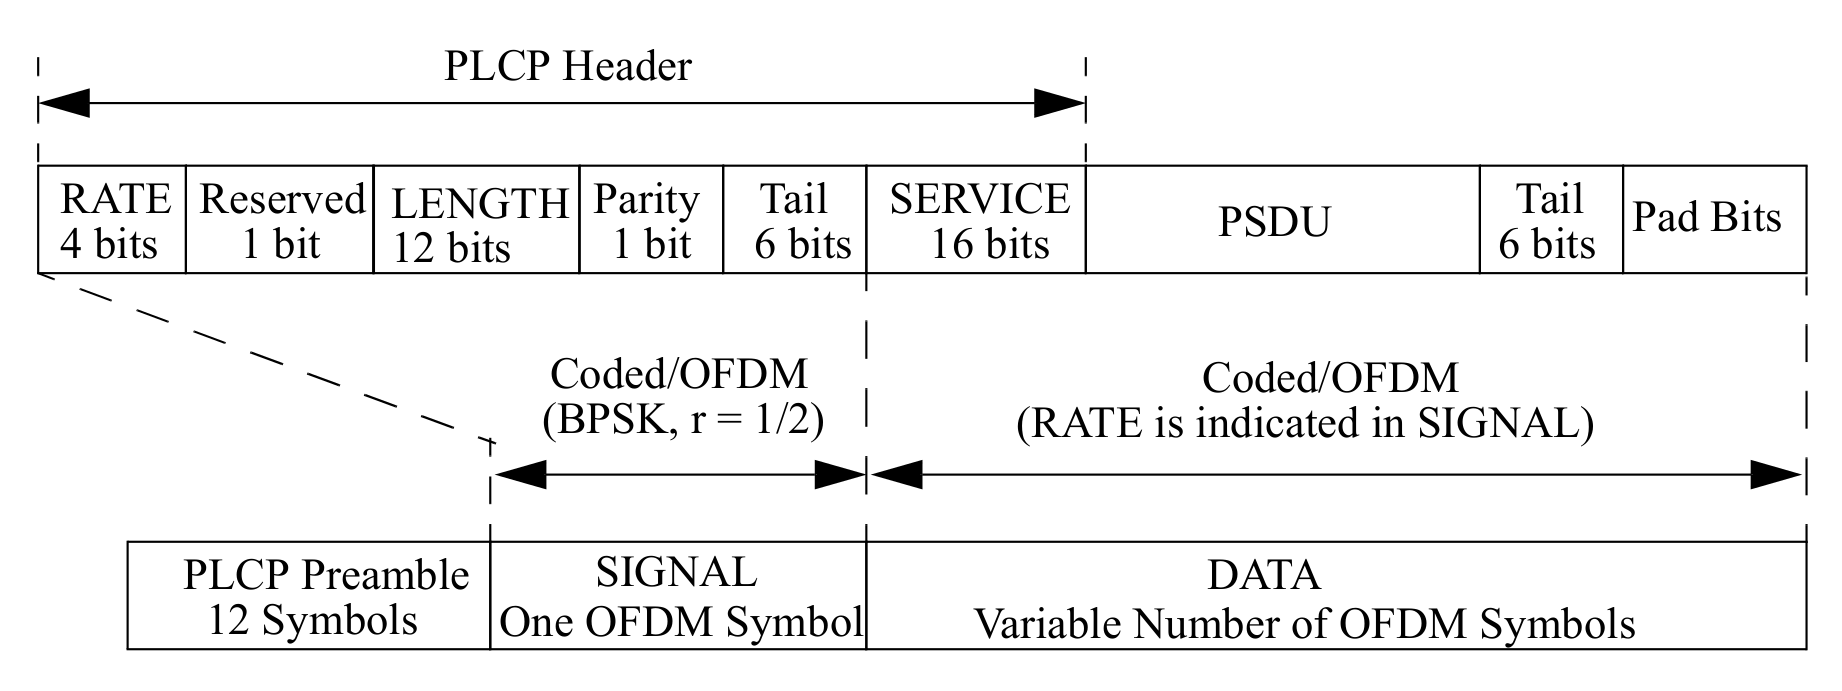
\includegraphics[width=\textwidth]{gfx/images/phy-format}
	\caption[\gls{IEEE} 802.11 Physical Layer Frame Structure]{\gls{IEEE} 802.11 Physical Layer Frame Structure \cite{ieee2012}}
	\label{fig:phy-format}
\end{figure}

After that, convolutional encoding is applied to the bits. The standard allows the encoder to use different code rates as specified by the \gls{MCS}. The encoder also uses a 7 bit state \cite{park2009}. Next, bits are grouped into symbols and rearranged using a deterministic permutation function \cite{perahia2013}. This is called interleaving. Following this, the symbols are modulated using \gls{QAM}	with different possible bit rates.\\

The available constellations are described by the modulation and coding scheme. Table \ref{tbl:mcs} shows all available \glspl{MCS} for \gls{IEEE} 802.11 a/g. Finally, pilot signals are added, the signal is transformed into the time-domain using the \gls{IFFT}, a cyclic prefix is added, and the signal is further processed and sent.

\begin{table}[ht]
	\centering
	\begin{tabular}{|p{2.5cm}|p{2.5cm}|p{2.5cm}|p{2.5cm}|p{2.5cm}|}
		\hline
		\textbf{MCS} & \textbf{Modulation} & \textbf{Coding Rate} & \textbf{Coded bits per symbol} & \textbf{Data bits per symbol} \\ \hline
		0 & BPSK & 1/2 & 48 & 24 \\ \hline
		1 & BPSK & 3/4 & 48 & 36 \\ \hline
		2 & QPSK & 1/2 & 96 & 48 \\ \hline
		3 & QPSK & 3/4 & 96 & 72 \\ \hline
		4 & 16QAM & 1/2 & 192 & 96 \\ \hline
		5 & 16QAM & 3/4 & 192 & 144 \\ \hline
		6 & 64QAM & 2/3 & 288 & 192 \\ \hline
		7 & 64QAM & 3/4 & 288 & 216 \\ \hline
	\end{tabular}
	\caption[\gls{IEEE} 802.11 a/g Modulation and Coding Schemes]{\gls{IEEE} 802.11 a/g Modulation and Coding Schemes (MCS) \cite{ieee2012} \label{tbl:mcs}}
\end{table}

The \gls{SIG}, which is transmitted before the Data Field, contains the \gls{MCS} used for the frame, and its length in octets. The Signal Field is always modulated with binary phase shift keying (BPSK) and rate $\frac{1}{2}$ \gls{BCC}. Nearby stations will also decode the \gls{SIG} to defer their transmissions for an appropriate time. The signal field has a duration of 4 $\mu$s.\\

In order to allow the receiver to calculate path effects of the channel, and to equalize received data, training fields are used in the beginning of the frame. The \gls{STF} is used for start-of-frame detection and \gls{AGC}. It includes 10 repetitions of a 0.8 $\mu$s symbol, resulting in a duration of 8 $\mu$s. The sequence is chosen to have good correlation properties and a low peak-to-average power, meaning its properties are preserved after clipping \cite{perahia2013}.

The \gls{LTF} is used for channel estimation, more precise frequency offset estimation, and time synchronization. It comprises 2 repetitions of a 3.2 $\mu$s training symbol, and 1.6 $\mu$s cyclic prefix, therefore the \gls{LTF} also spans 8 $\mu$s. Both training fields and the signal field form the preamble. Figure \ref{fig:preamble} shows detailed timing information for that.

\begin{figure}[H]
	\centering
	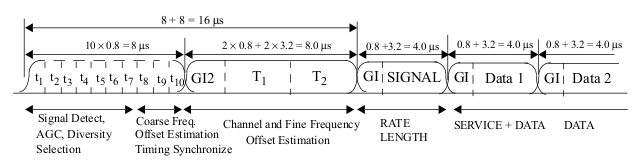
\includegraphics[width=\textwidth]{gfx/images/preamble-format}
	\caption[\gls{IEEE} 802.11 Preamble Timing]{\gls{IEEE} 802.11 Preamble Timing \cite{ieee2012}}
	\label{fig:preamble}
\end{figure}


\subsection{Medium Access Control Layer Specification} \label{sec:mac-format}

The Medium Access Control Layer (MAC) controls which station may transmit at a given time. The \gls{IEEE} 802.11 \gls{MAC} layer uses \gls{CSMA/CA}. With this algorithm, every station listens to the medium before a transmission. Collisions are prevented if possible, and detected through the lack of an acknowledgment packet. In contrast, Ethernet uses \gls{CSMA/CD}, where a transmitting station can directly sense a collision \cite{ieee802-3}.\\

A \gls{MAC} frame includes a \gls{MAC} header, a variable-length body, and a \gls{FCS} containing a \gls{CRC} Code.

The \gls{MAC} header consists of 2 byte frame control, 2 byte frame duration in microseconds, 18 bytes address 1, 2 and 3, as well some others depending on the frame control field. In a data frame, the address fields contain the receive address (RA), transmit address (TA), and the \gls{BSSID}. The frame structure is illustrated in figure \ref{fig:mac-format}.

\begin{figure}[H]
	\centering
	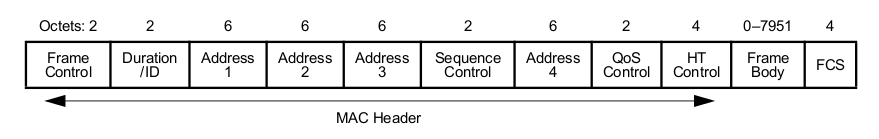
\includegraphics[width=\textwidth]{gfx/images/mac-format}
	\caption[\gls{IEEE} 802.11 \gls{MAC} Layer Frame Structure]{\gls{IEEE} 802.11 \gls{MAC} Layer Frame Structure \cite{ieee2012}}
	\label{fig:mac-format}
\end{figure}


%% -----------------------------------------------------------------------------

\section{Distributed Coordination Function}\label{sec:dcf}

The \gls{DCF} describes precisely when sending stations may transmit. It logically belongs to the \gls{MAC} layer. A station may send after sensing the medium idle for at least one \gls{DIFS} \cite{bianchi2000}. While a sender has access to the medium, it separates frames by a \gls{SIFS}, and other stations will not capture the medium because they must wait for a longer \gls{DIFS}.

After sensing the medium idle for a \gls{DIFS}, a station must wait a random backoff time before transmitting. This helps reduce collisions caused by multiple stations waiting to transmit. The backoff time is pseudo-randomly chosen out of the interval $[0..CW]$, where CW is the so-called contention window. On each unsuccessful transmit, CW is doubled. It is reset to its initial value as specified by the standard after a successful transmission.\\

The \gls{IEEE} 802.11 \gls{MAC} uses positive frame acknowledgements by layer 2 \gls{ACK} frames. Without an \gls{ACK} the sender retransmits the frame. To further reduce collision impact, large payloads are fragmented into multiple PSDUs, which are acknowledged individually. Data frames include a retry bit in the sequence number field to detect duplicate frames \cite{perahia2013}.\\

The hidden node problem can occur when a station sees the \gls{AP}, but not a third station that is currently transmitting to the \gls{AP}. The medium is busy, but the first station senses it as idle and begins a transmission. Therefore, the transmission to the \gls{AP} is subject to a collision. One approach to mitigate this is using an additional handshake mechanism before transmitting:

Before sending the data packet, a station transmits a \gls{RTS} Frame containing the desired sending duration. The access point will reply with a \gls{CTS} Frame, and third stations update a \gls{NAV} to remember the busy medium. In the hidden node scenario, the offending station would be able to receive the \gls{CTS} frame from the \gls{AP}, therefore knowing of the ongoing transmission. On top of that, \gls{RTS} frames are much shorter than data frames, meaning a collision is less harmful to the medium because less air-time is wasted.


%% -----------------------------------------------------------------------------

\section{Cross-Correlation}

The cross-correlation is a function of two continuous or discrete series that measures their similarity \cite{rabiner1978}. It is often used to compare different functions, or to search for a small feature in a larger stream of data.

With \gls{IEEE} 802.11, cross-correlation is applied to find the beginning of packets by correlating a known symbol of the short or long training field with a sample stream as captured by a receiver. However, in this thesis I will use it to also correlate the time-domain representation of \gls{MAC} addresses.\\

Since wireless transmission samples are discrete values, I disregard the continuous form of cross-correlation here. The discrete variant for series of samples f and g is calculated as follows:

$$ (f \star g)(n) = \sum_{m=-\infty}^{\infty} f^{\ast}(m) g(m+n) $$\vspace{0cm}

This formula is related to the convolution of the values, but it features the complex conjugate of the first function for the sum of products. A graphic analogy for cross-correlation would be sliding the functions against each other, where for each point all function values are multiplied individually and then added up.

In general, higher values of cross-correlations mean that the functions are more similar. It is worth noting that periodic functions have periodic cross-correlations, and that the \gls{IEEE} 802.11 Long Training Field is designed specifically in such a way that correlation is many orders of magnitude higher if the samples of two copies overlap exactly, than it is for any other alignment \cite{perahia2013}.


%% -----------------------------------------------------------------------------

\section{Multi-Path Channel Effects}\label{sec:multipath}

In an ideal scenario, a transmitted signal would travel on a direct line of sight from sender to receiver. However, electromagnetic waves spread in a spherical shape. In a real-world situation, signals can therefore reach the receiver on multiple paths, each affected by different delay, attenuation, reflection, or other effects.

A common multi-path effect are echoes, which are caused by signals being reflected on walls, furniture, or similar obstacles. When an echo occurs, an attenuated copy of the signal with a delay is received.\\

When trying to decode collisions, or detect affected senders, it is therefore important to take multi-path interference into account. Especially devastating is the fact that the signals add up at the receiving antenna. This means that the training fields in the preamble are affected by different paths and can hardly be used to calculate the inverted channel matrix. Chapter 5 provides more details on this problem.
